\section{M\'odulos adicionales}
Los m\'odulos adicionales son los encargados de dar funcionalidades al pipeline que hacen que mejore su rendimiento.

\subsection{Unidad de cortocircuito}
M\'odulo que se encarga de detectar si la instrucci\'on siguiente es dependiente de datos de la instrucci\'on anterior, es decir, si el resultado de la instrucci\'on es necesario por las instrucciones siguientes. En ausencia de este m\'odulo hay riesgos de lectura despues de escritura (LDE). En la figura \ref{fig:fwd} se muestra el m\'odulo.

\begin{figure}[H]
\centering
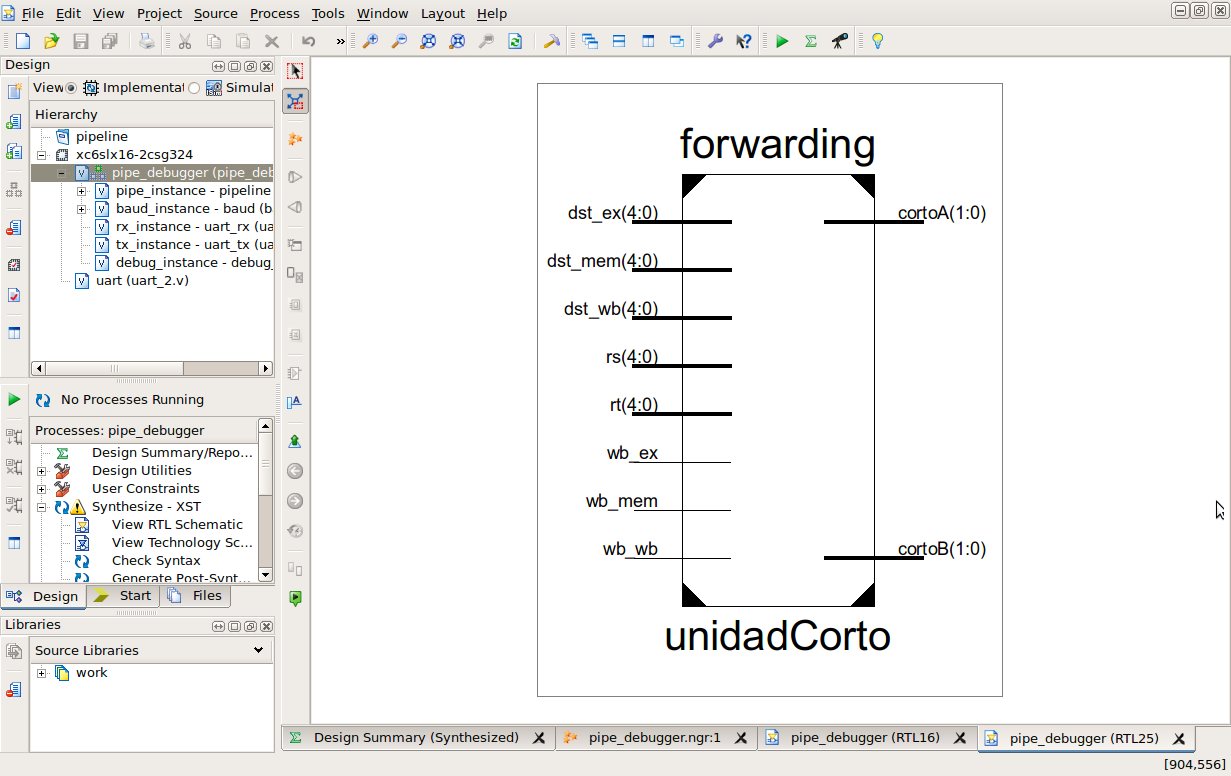
\includegraphics[scale=0.5]{img/forwarding}
\caption{Unidad de cortocircuito}
\label{fig:fwd}
\end{figure}

Tiene como entradas:

\begin{itemize}
  \item \textbf{dst\_ex}: Bus de 5 bits que proviene de la etapa de ejecuci\'on con el valor del registro que se va a escribir.
  \item \textbf{dst\_mem}: Bus de 5 bits que proviene de la etapa de memoria	con el valor del registro que se va a escribir.
  \item \textbf{dst\_wb}: Bus de 5 bits que proviene de la etapa de escritura con el valor del registro que se va a escribir.
  \item \textbf{rs}: Registros de la parte alta que se van a utilizar en la instrucci\'on que actualmente est\'a en la etapa de decodificaci\'on.
  \item \textbf{rt}: Registros de la parte baja que se van a utilizar en la instrucci\'on que actualmente est\'a en la etapa de decodificaci\'on.
  \item \textbf{wb\_ex, wb\_mem, wb\_wb}: Señales de wb que salen de los latchs de cada una de las etapas siguientes para avisar que se va a escribir un registro.  
\end{itemize}

Las salidas del m\'odulo son:
\begin{itemize}
  \item \textbf{cortoA}: Bus de 2 bits que indica si se produjo una dependencia de datos y entra a un multiplexor para que se elija el valor correspondiente cortocircuitado de la etapa en que se detecta el uso de un registro en riesgo, para insertarlo en la parte baja de los datos que salen del banco de registros. 
  \item \textbf{cortoB}: Bus de 2 bits que indica si se produjo una dependencia de datos y entra a un multiplexor para que se elija el valor correspondiente cortocircuitado de la etapa en que se detecta el uso de un registro en riesgo, para insertarlo en la parte alta de los datos que salen del banco de registros.
\end{itemize}

\subsection{Detector de riesgo}

Este m\'odulo se encarga de actuar en la etapa de decodificaci\'on, impidiendo la carga y lectura de una nueva instrucci\'on. Para que se de este caso, la instrucci\'on en la etapa de ejecuci\'on debe ser del tipo load y el registro de destino del load debe coincidir con el registro de la siguiente intrucci\'on. Si se dan estas condiciones, entonces existe riesgo y es necesario parar el pipeline insertando una burbuja. El m\'odulo se muestra en la figura \ref{fig:datahazard}.

\begin{figure}[H]
\centering
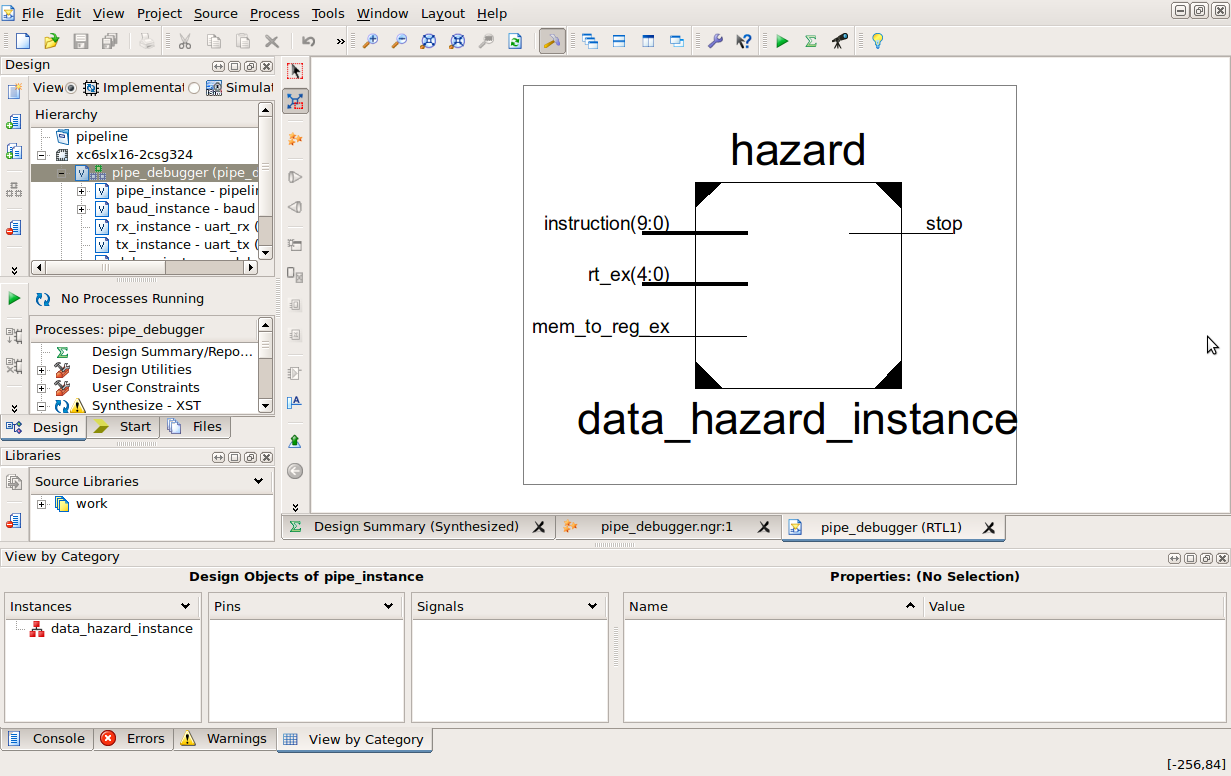
\includegraphics[scale=0.35]{img/data_hazard}
\caption{Detector de riesgo}
\label{fig:datahazard}
\end{figure}  

Las entradas a este m\'odulo son:
\begin{itemize}
  \item \textbf{instruction}: Bus de 10 bits en donde se encuentran los dos registros que pueden sufrir un riesgo a causa de un load.
  \item \textbf{rt\_ex}: Registro que la instrucci\'on del load va cargar.
  \item \textbf{mem\_to\_reg\_ex}: Señal que alerta que se va a cargar un registro desde memoria. 
\end{itemize}

La salida es una señal de \textbf{stop} que va a ser utilizada en el contador de programa para que este no avance y en el latch entre la etapa de b\'usqueda y decodifici\'on. 